% Created 2023-02-19 Sun 10:49
\documentclass[9pt, b5paper]{article}
\usepackage{xeCJK}
\usepackage[T1]{fontenc}
\usepackage{bera}
\usepackage[scaled]{beraserif}
\usepackage[scaled]{berasans}
\usepackage[scaled]{beramono}
\usepackage[cache=false]{minted}
\usepackage{xltxtra}
\usepackage{graphicx}
\usepackage{xcolor}
\usepackage{multirow}
\usepackage{multicol}
\usepackage{float}
\usepackage{textcomp}
\usepackage{algorithm}
\usepackage{algorithmic}
\usepackage{latexsym}
\usepackage{natbib}
\usepackage{geometry}
\geometry{left=1.2cm,right=1.2cm,top=1.5cm,bottom=1.2cm}
\usepackage[xetex,colorlinks=true,CJKbookmarks=true,linkcolor=blue,urlcolor=blue,menucolor=blue]{hyperref}
\newminted{common-lisp}{fontsize=\footnotesize} 
\author{deepwaterooo}
\date{\today}
\title{ET}
\hypersetup{
  pdfkeywords={},
  pdfsubject={},
  pdfcreator={Emacs 28.2 (Org mode 8.2.7c)}}
\begin{document}

\maketitle
\tableofcontents


\section{ET框架框架设计模块功能等}
\label{sec-1}
\subsection{一个双端框架的12个项目,目录结构}
\label{sec-1-1}
\begin{itemize}
\item 就不知道这12个项目是如何组织构建起来的
\end{itemize}
\subsubsection{客户端的四个项目}
\label{sec-1-1-1}

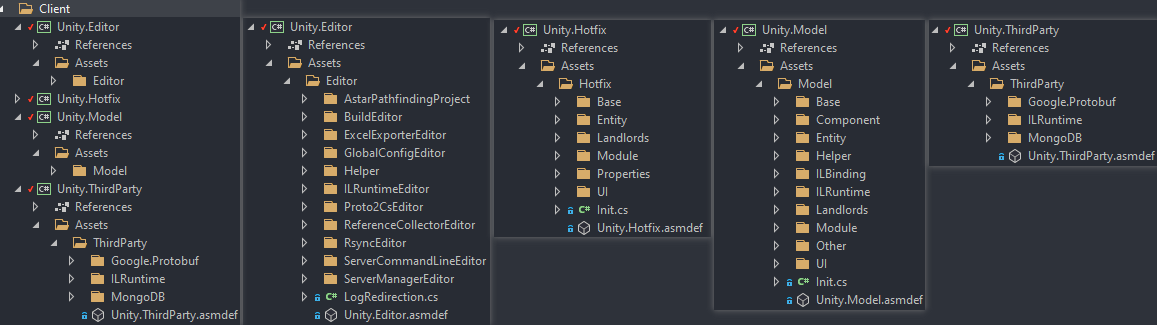
\includegraphics[width=.9\linewidth]{./pic/readme_20230201_200218.png}
\subsubsection{服务器端的8个项目:}
\label{sec-1-1-2}

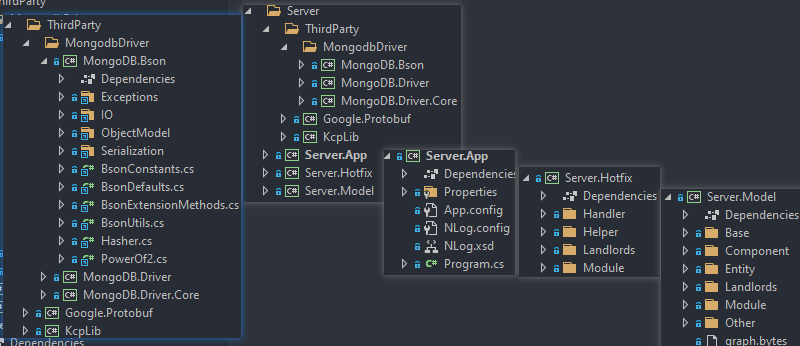
\includegraphics[width=.9\linewidth]{./pic/readme_20230201_201117.png}
\begin{itemize}
\item ET-EUI整理出了一个小小的登录系统,如果这个系统能够运行得通,配置简单顺利,也就基本上也算是达到自己小小服务器的需要了。运行一下试试看。
\end{itemize}
\subsection{模块功能管理}
\label{sec-1-2}
\subsubsection{ET框架中事件使用的规则和注意事项}
\label{sec-1-2-1}
\begin{itemize}
\item \textbf{事件结构体的定义} 必须在Model或ModelView下, \textbf{事件的订阅和发布} 必须在Hotfix或HotfixView下 (是否为View层根据是否需要UnityAPI决定)
\item 在ET框架中 \textbf{View层可以直接调用逻辑层的代码} ,而 \textbf{逻辑层不允许直接调用View层的代码} ,所以逻辑层想要和View层交互只能使用抛出事件的方式,让View层进行订阅进行相应的处理。
\end{itemize}
\subsubsection{ET框架下ETTask的异步编程}
\label{sec-1-2-2}
\begin{itemize}
\item 开发早期都是使用协程或者多线程进行程序异步的实现,
\item 在C\#5.0之后引入了Tasync await等关键字可以轻松优美的实现程序的异步进行。
\item Task是C\#异步编程库的异步功能基础类型,包含了多线程的使用。
\item 而ET框架主打的是 \textbf{多进程单线程} ,所以使用ETTask对Task进行了封装,使其不用考虑多线程的共享难题,更易于使用。
\end{itemize}
\subsubsection{协程}
\label{sec-1-2-3}
\begin{itemize}
\item 协程其实就是创建一段程序辅助主线程的运行,注意 \textbf{协程不是多线程,其仍运行在主线程当中,其只是将一个函数按照一定的条件分解成若干块,穿插在主线程的各个位置中运行。}
\item async 和 await关键字
\begin{itemize}
\item async是修饰函数的关键字,被修饰的函数称为异步函数,只有被此关键字修饰的函数才能使用await关键字
\item await关键字后跟一些表达式(一般是返回值为ETTask的函数),在异步函数运行到此时会立即跳出函数,继续执行原逻辑。
\item await返回前会做出保证,保证await后表达式的任务完成后,执行点会跳回异步函数中,继续向后执行剩余代码
\item 若await后表达式正常返回,可用变量接收表达式的返回值,表达式的返回值类型为定义表达式ETTask<>的泛型
\end{itemize}
\end{itemize}

\section{小小服务器:要怎么才能开始动手试图去实现这个小服务器呢?}
\label{sec-2}
\subsection{如果适配ET框架,现游戏可能哪些模块版块存在问题}
\label{sec-2-1}
\begin{itemize}
\item 我也觉得ET框架可能不太适合我现在的游戏(也就是说,把我的游戏完全适配成ET框架来开发,原本只需要一个小小服务器,完全适配为ET框架,就把问题弄得狠复杂了。。。),
\item 使用ET框架,我所有的安卓基础就会被抛到九宵去外,不再关安卓SDK  NDK什么事儿了。。。。。是对自己太大的损耗。而我原本还可以简单封装实现的安卓录屏,游戏内使用安卓SDK相关功能模块录屏游戏过程等,会被全部废掉,损失太大不值得。我觉得我就只要个文件服务器加个数据库而已。
\item 原因是:我现在还想不通若是用ET框架来实现自己游戏的(服务器与客户端双端都可以热更新),我该如何实现我的方块砖10个按钮上的点击事件,射线检测?它的ILRuntime热更新程序域里对射线检测包的组件安装可能会成为自己狠大的问题,因为还不是狠懂里面的内部原理.这个模块重构的原理是:把射线检测,如果必要一定要,封装成如ET中任何其它可装载卸载的组件一样的装载到某个必要场景上去.
\begin{itemize}
\item ET里有个检测鼠标左右键位置的帮助类,但跟射线检测应该还是相差狠远的.而游戏场景里面有一个OperaCompoent,这个组件会实时监听按键的点击并且将点击的位置发送给服务器,服务器再传送回客户端
\end{itemize}
\item 所以,现在对这个框架,最深的感触是:盲人摸象,摸每部分细节似乎都快清楚了,却无法组装从一个更高的层面上来理解和把握框架设计,无法吃透,在大框架功能模块上犯难,在网上再搜一搜
\item 我可以把两组按钮画面同样做成预设与热更新资源包,射线检测同样会成为可装载可卸载的组件,可是再后面射线检测到的物体逻辑,感觉有点儿复杂了
\item 
\end{itemize}
\subsection{如果不适配,怎么弄个服务器带数据库等逻辑?}
\label{sec-2-2}
\begin{itemize}
\item 使用部分共享源码的双端(共享的是文件服务器8个项目,MongoDB数据库服务器, Realm注册登录用,网关服,Location服, ETTAsk, RPC消息机制, NetComponent等自己机对陌生需要练习,而自己的服务器也不可缺省的相关功能)
\item 现在知道自己整的不沦不类的服务器所谓的登录,登录的是网页上的认证相关,跟自己真正要实现的游戏里注册登录服保存数据库完全两回事,现在知道了。
\item 作用ET的头,实现用户注册与登录,适配自己现有游戏的尾,游戏除了入口之外全游戏进热更新程序域里
\item 那么自己的现框架架构作尾,全游戏逻辑进热更新域,存在的问题就变成是:
\item 我无法再实时动态检查用户上下线顶号之类的,我只能默认登录过就是登录状态,可是用户下线了,或更严格的说掉线了,服务器并不及时知道,可以通过安卓SDK中的按钮登出知道。但是掉网了掉线了呢?(这部分的逻辑可以晚点儿再考虑,把网络请求相关的摸得再熟悉一点儿再弄)
\item 再则,ILRuntime热更新程序域里,我又该如何实现在热更新程序域里网络上载用户的游戏保存进展?这里需要去想和理解,为什么它ET框架就可以在热更新程序域里同网络交互,你哪里还没有想明白?
\item ET框架,热更新程序域里装载的组件,只是帮助与外界游戏程序域连通好,真正的网络请求上传下载等是在热更新域外面完成链接式传进去的?感觉对这个大框架没有掌握好,脑袋仍然是在像糊糊一样。。。
\item ET框架,网络的那部分做得还是比较完整的。实现在了各种的封装,涉及大量的网络调用与交互,游戏过程中的交互与更新。但是太多的功能对于自己的游戏来说完全不必要.所以只想用ET的头
\item 各种泛型,接口的定义,一二三个参数等的泛型接口定义(你可以去找一找工程中的各种ILRuntime的适配器),全都是都可以成为热更新域里能够被游戏程序域里识别的原因,所以狠多设计,自带ILRuntime的适配性质
\item 那么就可以小一点儿一点儿地来,先弄个登录窗口,实现服务器的注册登录保存登录信息到数据库,相对比较小点儿的逻辑.这个过程中把MongoDB数据库的配置等所有连接过程中必要的步骤,可能出现的问题给解决掉,就算前进了一小步呀
\item 不知道怎么开始,也不知道怎么创建可以㠌套的像是安卓模块库一样的子工程,就只能把小游戏斗地主复制一份了再从它的基础上来改?!!!
\item 如果简单一点儿开始,我觉得我应该是可以先把简单点儿的MongoDB数据库连接成功,把用户登录相关的逻辑,网络交互的部分,ETTask RPC ACTOR消息等,哪怕是复制,把这部分弄过去
\end{itemize}
\subsection{ET框架}
\label{sec-2-3}
\begin{itemize}
\item \url{https://blog.csdn.net/qq_33574890/article/details/128244264?spm=1001.2101.3001.6650.1&utm_medium=distribute.pc_relevant.none-task-blog-2\%7Edefault\%7EAD_ESQUERY\%7Eyljh-1-128244264-blog-123841252.pc_relevant_multi_platform_whitelistv4&depth_1-utm_source=distribute.pc_relevant.none-task-blog-2\%7Edefault\%7EAD_ESQUERY\%7Eyljh-1-128244264-blog-123841252.pc_relevant_multi_platform_whitelistv4&utm_relevant_index=2} 上次看看得不是狠懂,这次再看,至少是觉得UI的逻辑处理,作者的观点更自然真实一些,放在一个文件一起处理,个人认为更好,而不是折分成为几个文件 
\begin{minted}[fontsize=\scriptsize,linenos=false]{csharp}
class LoginState:State{
	void OnEnter(){
		UI.Show()
	}
	void OnLeave(){
		UI.Hide()
	}
}
\end{minted}
\end{itemize}

\section{登录协议流程}
\label{sec-3}
\begin{itemize}
\item 因为登录协议是客户端与服务器通信的,不属于服务器内部协议,所以打开OuterMessage.proto,里面存放的都是客户端与服务器通信定义的协议数据。
\item 比如定义如下,登录协议:
\end{itemize}
\begin{minted}[fontsize=\scriptsize,linenos=false]{text}
message C2G_LoginGate // IRequest
{
	int32 RpcId = 90;
	int64 Key = 1;	// 帐号
}

message G2C_LoginGate // IResponse
{
	int32 RpcId = 90;
	int32 Error = 91;
	string Message = 92;
	int64 PlayerId = 1;
}
\end{minted}
\begin{itemize}
\item emacs里org-mode exporte-to-pdf希望有个latex选择可以自动将\^{}I转化为空格,而不是这种字符,晚点儿再弄这个
\item 注意点: \textbf{没有意识到像是注释一样的片段,这个协议里,会成为标注或是标签}
\begin{itemize}
\item 1.因为登录是请求-响应类型协议(即发送一条数据,并期望返回一条数据),所以注意对应C2R\_Login协议带有“//ResponseType R2C\_Login”标志,在生成协议时,用于标记这个C2R\_Login请求对应的响应类型为R2C\_Login
\item 2.因为请求是直接发送给realm服的,所以是普通的IRequest类型协议,标记为IRequest
\item 3.R2C\_Login回复类消息结构,因为是Realm服发送给客户端的,因此是一个普通IResponse
\item 4.注意两个协议类里面都有RpcId,主要用于发送请求-响应类消息时,发送将自己的RpcID发送出去,返回时带回这个值,用于发送方接受到返回协议时,可以找到对应的是哪一个请求协议返回来的。
\end{itemize}
\end{itemize}

\section{一步一步的进展 }
\label{sec-4}
\begin{itemize}
\item 现在还是不想这么改,因为项目太大了,搞不清哪是哪里,另外狠多类是部分类,就是一个类可以有好几个地方来定义扩展这个类,然后同样好几个同样的类,就不知道该在哪个类里定义。12个项目之间的交互有点儿复杂,现在没有吃透,只适合小范围改动去帮助自己理解项目,还不适合自己从头到底来重构自己的项目。就按网络上的建议,先把注册登录系统的逻辑再修改一遍,直接再接自己的热更新程序域
\item 再往下走。因为接自己项目的入口就全进自己项目的热更新域仍然存在诸多的登录登出掉线,以及用户游戏进展数据的保存等相关逻辑。可是因为急需要下手练习,顾不上这么多,先练再说,练到哪里是哪里。。。。。
\item 首先,把斗地方大厅改写为游戏主菜单的三个选项(如果我只想用ET的头,它的头太大了,还是要自己弄个小小的头,小小的服务器,所以暂时就还是考虑自己从头实现一个MongoDB的小小服务器比较容易一点儿,不懂的就翻ET)
\end{itemize}

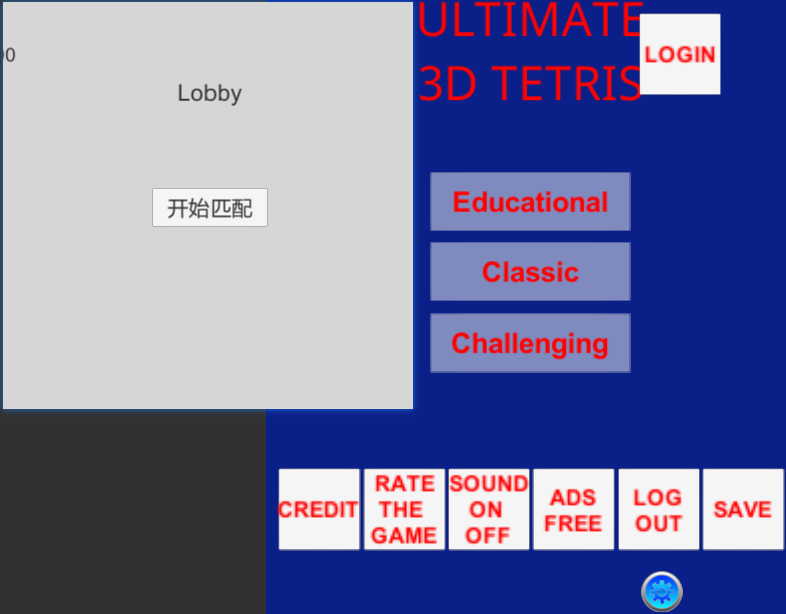
\includegraphics[width=.9\linewidth]{./pic/readme_20230201_202642.png}
\begin{itemize}
\item 把这个界面的相关上下文全部适配好:UI的自动创建生成系统,UI的按钮点击回调等
\item 这里想要找的是: 在点击的回调里如何,是否可以卸载装载UI组件,还是说必须得去HotfixView 什么视图层来处理这些逻辑呢?
\end{itemize}
\subsection{UIType.cs: 这种类型的定义好像不止加一个地方,一个地方不够,可是大的框架架构还是没搞明白}
\label{sec-4-1}
\begin{minted}[fontsize=\scriptsize,linenos=false]{csharp}
namespace ETHotfix {

    public static partial class UIType {
        public const string Root = "Root";
        public const string UILogin = "UILogin"; // 注册 登录 界面
        public const string UILobby = "UILobby"; // 主菜单 三选项

// 上面的界面远远不够呀。。。
        public const string UIEducationalMode = "UIEducationalMode"; 

        public const string UIEducational = "UIEducational"; 
 // 怎么再把它细化为:三 四 五方格呢? 应该是要用同一接口的不同实现,完全重复写三个系统会把人弄死的。。。。。
        public const string UIGridThree = "UIGridThree";
        public const string UIGridFour = "UIGridFour"; 
        public const string UIGridFive = "UIGridFive"; 

        // 那么就涉及游戏界面的折分:哪些是可以公用,哪些是不得不细化最小粒度的?
        
        public const string UIClassic = "UIClassic"; 

        public const string UIChallenge = "UIChallenge"; 
 // 挑战难度:要定义接口来实现20-50个不同的实现了?        
    }
}
\end{minted}

\begin{itemize}
\item 安卓SDK这个框架其实并不受影响。但本质是所有安卓SDK的东西不能够热更新。因为ET是网络多人游戏框架的,可能更多的是不适合添加与适配案桌SDK。这些晚点儿再得结论好了,反正我的案桌SDK本质也是可要可不要。如果能够快速掌握一个比较好的双端框架的话
\item 不知道若是照这么改下去,得把这个游戏改成是什么花葫芦呢?
\end{itemize}
\section{带MongoDB数据库的注册登录用户帐户管理资源文件服务器}
\label{sec-5}
\begin{itemize}
\item 去找和实现简单的服务器项目,操纵MongoDB数据库
\item 除了自己的电脑安装有MongoDB数据库之外,服务器项目中因为要连接操纵电脑上数据库,可能还需要狠多插件的安装与配置,连接字符串,什么MongoDBClient之类的。这些细节就只能找到一个小参考项目,自己试着连接,出错了再一一更正自己可能存在的错误,要真正能够把项目连通运行得起来,才算真的解决问题
\item 
\end{itemize}
\section{ET框架-19 ET框架账号中心服逻辑编写(1)}
\label{sec-6}
\begin{itemize}
\item \url{https://blog.csdn.net/m0_48781656/article/details/124899665?spm=1001.2101.3001.6650.1&utm_medium=distribute.pc_relevant.none-task-blog-2\%7Edefault\%7ECTRLIST\%7ERate-1-124899665-blog-123592622.pc_relevant_multi_platform_whitelistv3&depth_1-utm_source=distribute.pc_relevant.none-task-blog-2\%7Edefault\%7ECTRLIST\%7ERate-1-124899665-blog-123592622.pc_relevant_multi_platform_whitelistv3&utm_relevant_index=2}
\item 现在,对ET 框架里,热更新层,不变层的大的框架层次,稍微开始有点儿概念。还需要再多理一理。现在觉得,只要自己感兴趣,想要找的逻辑都能够找得出来。只是还需要多运行几遍帮助理解消化。
\item 但是现在什么都有了,应该能够很好地实现 ET 的头加自己项目的主体部分了。客户端的逻辑基本都懂了,服务器端需要明天上午再看一下
\item 只是仍需要考虑,将来如何自己写个多人小游戏?
\end{itemize}
\section{ET 框架登录流程}
\label{sec-7}
\begin{itemize}
\item 1.服务器由于在启动时就添加了NetOuterComponent组件,默认状态下使用Tcp协议,组件启动时,指定了自己的消息解析器为ProtobufPacker,消息派发器为OuterMessageDispatcher。
\item 2.由于NetOuterComponent继承了NetworkComponent,然后在awake里,调用了NetworkComponent的Awake方法。
\item 3.实例化一个TService,并监听启动端口,绑定OnAccept。
\item 4.当客户端的协议通过端口与IP发送C2R\_Login协议时,TService监听到一个新的连接,在底层建立一个TChannel(内部封装了socket)与之关联,回调OnAccept。
\item 5.OnAccept回调新建一个Session,并将建立的TChannel与这个Session关联起来,并启动Session,内部会调用TChannel的Socket启动循环获取数据。
\item 6.底层Socket获取数据会通知TChannel进行处理,进而将处理好的流数据回给Session的OnRead进行序列化,协议号解析等操作。
\item 7.消息类型为IRequest,所以直接交给OuterMessageDispatcher协议消息转发器进行处理。
\item 8.OuterMessageDispatcher发现是非Actor消息,调用MessageDispatcherComponent组件直接对消息进行处理。
\item 9.由于C2R\_LoginHandler类之前就已经在MessageDispatcherComponent注册好,所以C2R\_Login消息直接交给他处理。
\item 10.首先应该根据数据库进行帐号密码验证(这一步ET在DEMO中省略了),然后根据配置,拿到一个随机的Gate服务的端口与地址,通过内网组件NetInnerComponent拿到一个通向该地址与端口的Session。然后Reaml模块向Gate模块发送一个R2G\_GetLoginKey,为客户端请求一个唯一Key当作连接GATE时的鉴权,这里使用了异步await。 \textbf{注:在ALLSERVER模式下,没有区分Reaml模块与Gate模块,但实际流程是一样的。}
\item 11.身为Gate服务模块的NetInnerComponent会监听自身提供的端口,同样的Session会将消息解析好之后发给NetInnerComponent的MessageDispatcher(即InnerMessageDispatcher)进行处理。
\item 12.InnerMessageDispatcher发现R2G\_GetLoginKey是一个普通IRequest消息,因此直接交给MessageDispatcherComponent的Handle进行处理。
\item 13.同样的R2G\_GetLoginKeyHandler类也注册好了,直接到R2G\_GetLoginKeyHandler的Handle方法中,由于R2G\_GetLoginKeyHandler继承自AMRpcHandler,在AMRpcHandler中,构造了一个Reply函数传给Run方法,同时也将Response实例化(这里是G2R\_GetLoginKey类实例)传给Run。
\item 14.R2G\_GetLoginKeyHandler实现了Run方法,Run方法处理R2G\_GetLoginKey。他会随机一个64位的数放入到G2R\_GetLoginKey的返回数据中,并调用Reply。
\item 14.Reply内部会调用NetInnerComponent一路传过来的Session进行Session的Reply方法调用,直接将G2R\_GetLoginKey发送回去。
\item 15.Reaml与Gate连接的Session收到了数据,由于是G2R\_GetLoginKey是IResponse类协议,所以不走MessageDispatcher转发了,直接走之前发送时注册的回调函数处理
\item 16.回调函数内部是直接将异步TCS设置SetResult,来唤醒回调,这样一步步向上唤醒最终回到第10步中的await处。
\item 17.可以看到C2R\_LoginHandler也是继承自AMRpcHandler,所以再AMRpcHandler内也封装了一个reply回调,以及一个R2C\_Login实例传给C2R\_LoginHandler的Run,现在回到await处。
\item 18.通过配置拿到Gate服务模块的外网OuterConfig的Address2,以及上面回来的Key,传给response,调用reply通过session将消息发出去。
\item 19.同样的方式,客户端收到一个IResponse,调用之前Call发送数据时注册好的回调,回调内部设置tcs.SetResult,唤醒异步方法。从而回到客户端发送请求的await处。
\item 20.客户端拿到请求后,通过发来的Address新建一个与Gate的连接,然后发送C2G\_LoginGate
\item 21.Gate服务收到协议后,通过一系列底层转发,周转到C2G\_LoginGateHandler类进行处理。
\item 22.验证成功后,Gate为每个玩家新建一个Player实体与之对应,并交给PlayerComponent进行管理,同时将与之关联的Session上挂载SessionPlayerComponent,将实体Player与关联的Session关联起来,最后为关联的Session绑定一个MailBoxComponent。这样Gate的内网组件就能将Actor消息转到这个Session进行处理时,可以直接当entity为这个session进行转发即可,注意Player基类为ComponentWithId,所以Player的ID即为他的InstanceId。同时将这个ID发回给客户端,当作唯一ID来使用(猜测是在Gate上的实体,不会发生转移的原因)。
\item 自此,客户端已经完整的登录到Gate,后续客户端的通信全部与GATE进行通信,Gate对客户端协议进行转发,收到其他服务传过来的Actor消息,也能转发到对应的客户端Session进行处理。
\item 用一个图来表达的话,就成为下面的样子:也是网友总结的:
\end{itemize}

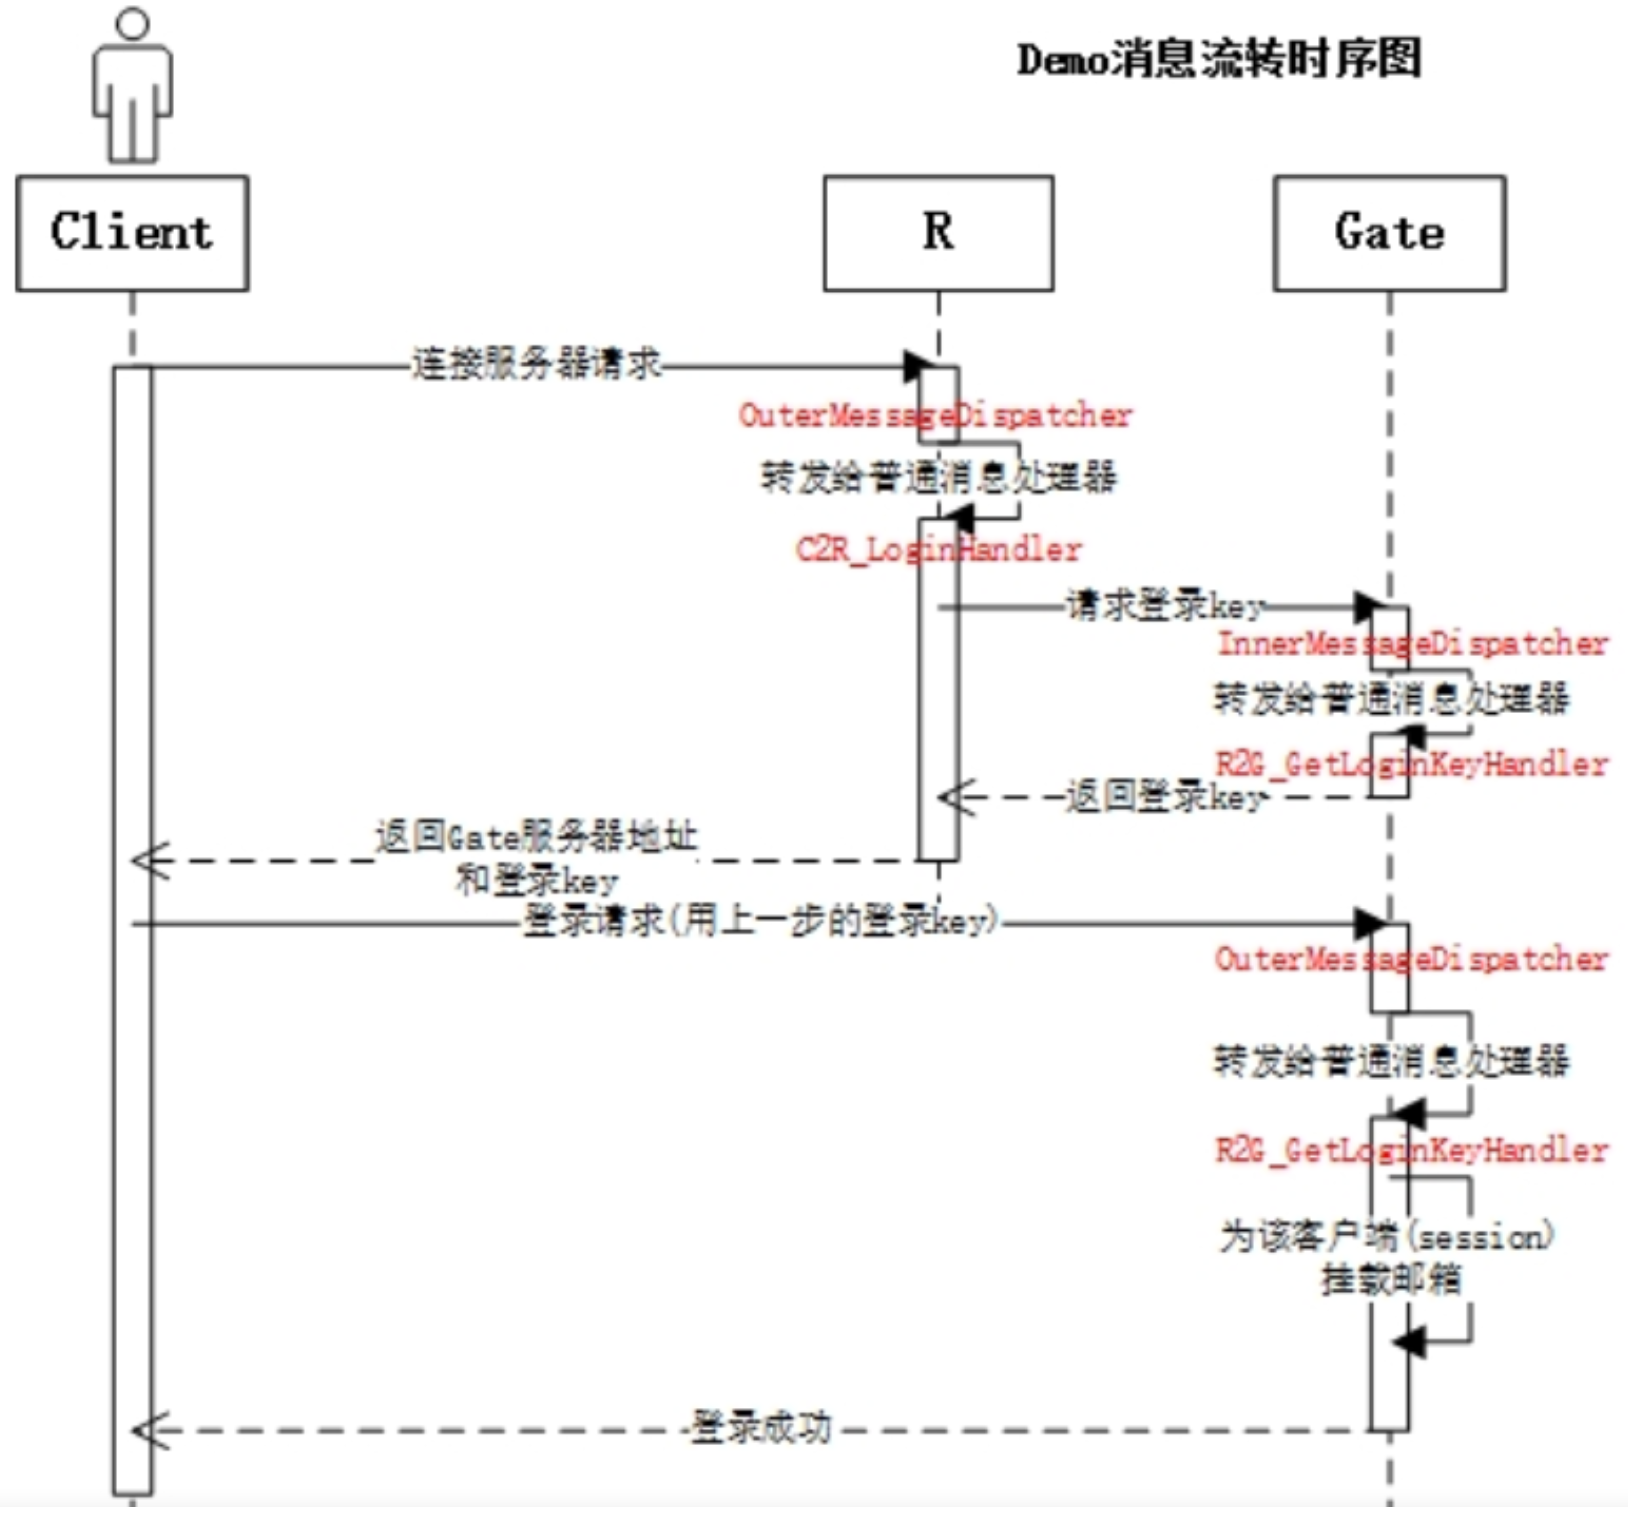
\includegraphics[width=.9\linewidth]{./pic/readme_20230219_104114.png}
\section{与其他服务模块通信基础(以Map服为例)}
\label{sec-8}
\begin{itemize}
\item 客户端想要进入其他服务模块,首先都会再该服务上创建或者移动一个实体进去。
\item 这里以与Map服通信为例。
\begin{itemize}
\item 1.客户端向Gate发送一条C2G\_EnterMap协议,GATE收到服务的细节这里就不多说一遍了,由于C2G\_EnterMap是IRequest,所以最终由C2G\_EnterMapHandler类进行处理。
\item 2.通过与之关联的Session上SessionPlayerComponent,能拿到在Gate上的Player信息。然后再通过配置拿到一个Map服务的地址,通过NetInnerComponent在Gate上构建一个与选好的Map服务进行通信的Session。
\item 3.向这个Session发送一条G2M\_CreateUnit协议,将Gate上的player实体ID,session的InstanceId都发送过去。
\item 4.经过底层处理后,由G2M\_CreateUnitHandler类处理,首先创建一个Unit实体, \textbf{与在Gate上创建Player实体不同,Player的ID赋值为组件的InstanceID,而在Map上的Unit实体,通过IdGenerater.GenerateId()方法生产一个唯一ID作为实体的Id。}
\item 5.给Unit上添加移动,寻路组件,并给一个初始化的位置,并为其添加一个MailBoxComponent代表这个unit为一个Actor。由于在Map上的Unit会发生转移到其他服务模块上的可能,所以需要通过MailBoxComponent的AddLocation方法,向Location服务模块,注册自己的唯一ID,与自己的InstanceId。
\item 6.通过NetInnerComponent获取一个与Location服务连接的Session,并发送一个ObjectAddRequest协议,经过一系列处理后,在Location服务上由ObjectAddRequestHandler类处理,调用LocationComponent的Add将ID与InstanceId注册好,然后直接返回。
\item 7.Map服务上收到Respose,Session唤醒异步,回到第5步,注册好定位服务(Location)后,给Map上的Unit添加一个UnitGateComponent组件,将Gate发过来的Gate与客户端连接的Session实例ID给保存到Unity上。
\item 8.将这个Unit放入到UnitComponent组件中进行管理。将生成的唯一Unit ID添加到回复的response协议中。
\item 9.创建一条M2C\_CreateUnits协议,查询UnitComponent组件,遍历所有已经存在的Unit,将数据添加到createUnits协议数据中,广播M2C\_CreateUnits协议。
\item 10.M2C\_CreateUnits协议类型是IActorMessage,进入MessageHelper,获取所有的Unit,获取到ActorMessageSenderComponent组件。
\item 11.遍历所有unit,获取unit上UnitGateComponent组件获取连接状态,通过actorLocationSenderComponent以及每个Unit上挂载的unitGateComponent的GateSessionActorId,这个值是创建Unit时,存储的从GATE上与客户端连接的Session的InstanceId。
\item 12.因为在GATE上的实体不会发生转移,所以他的InstanceId很稳定(个人觉得也可以拿GATE上Player的InstanceId做后续处理),通过InstanceId即可拿到对应生产他的Gate的端口与地址,通过端口与地址,新建一个ActorMessageSender实例。
\item 13.通过actorMessageSender发送上面的广播协议,通知所有客户端新的实体被增加了。这里实际走的是向Gate发送了一条IActorMessage协议,然后Gate内网组件收到,转给InnerMessageDispatcher处理,再转给mailBoxComponent处理,然后调用到MailboxGateSessionHandler,将协议转发给客户端即可。 \textbf{备注:这里有个小处理:iActorMessage.ActorId = 0,不暴露内部参数}
\item 14.广播通知所有客户端生成了一个新的Unit后,回复一个M2G\_CreateUnit。
\item 15.再次经过一系列处理后,Gate服务收到M2G\_CreateUnit,依然是由Session唤醒异步到Gate的C2G\_EnterMapHandler的创建请求处。
\item 16.将创建好的UnitId即Map上的Unit这个唯一ID(注:与InstanceId不同,他是在Location中绑定过的),绑定到Gate上Player的UnitId上,同时赋值给G2C\_EnterMap协议中,发回给客户端。这样后面Gate进行双向转发时,都能通过这个UnitId来进行。
\end{itemize}
\item 自此,创建好Map上Unit,绑定了UnitId,在Location上注册了Map上的Unit,便于发送ActorLocation协议
\end{itemize}

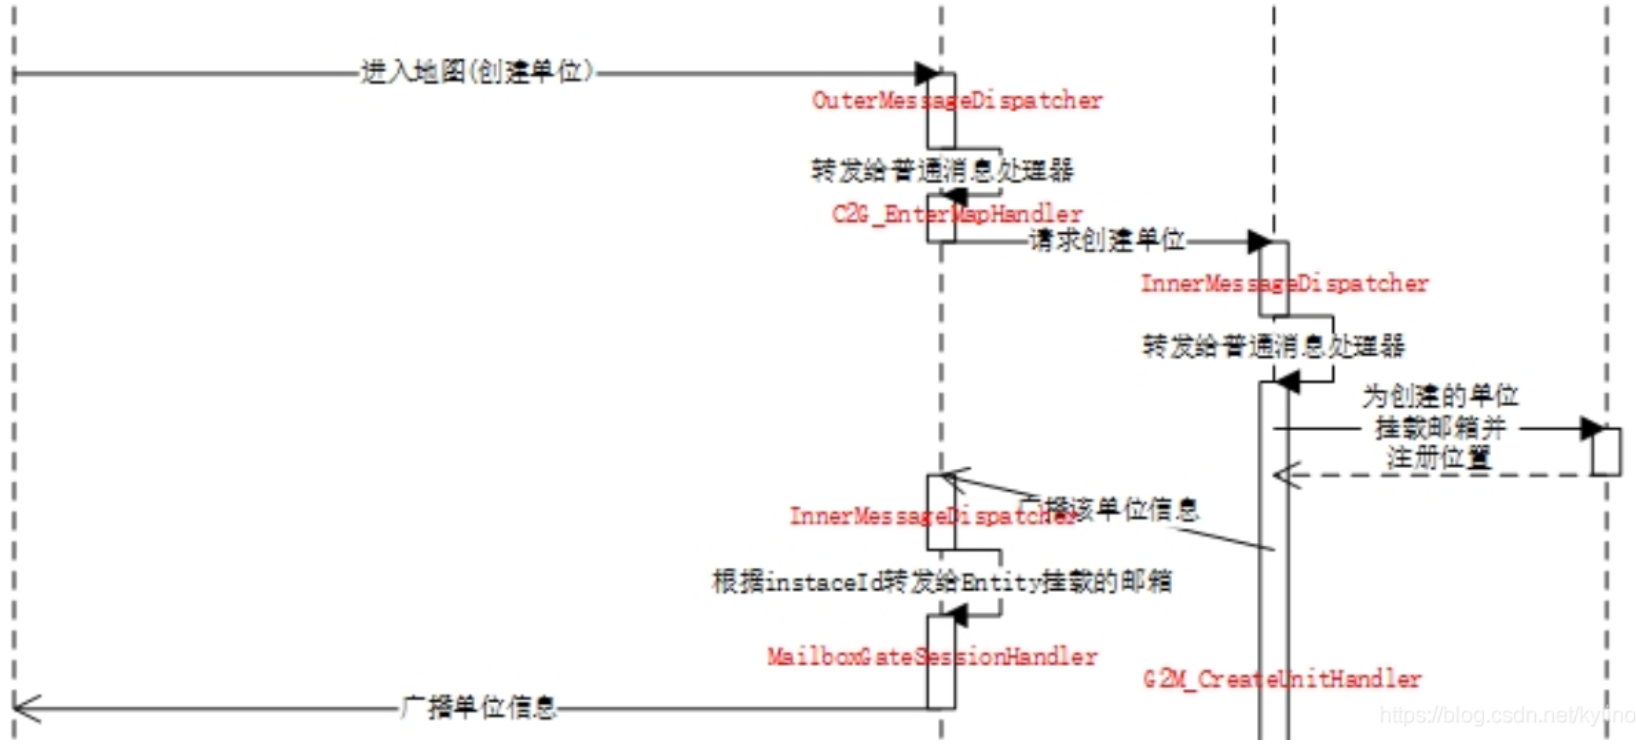
\includegraphics[width=.9\linewidth]{./pic/readme_20230219_103732.png}
\section{与其他服务模块通信Actor(以Map服为例)}
\label{sec-9}
\begin{itemize}
\item 现在客户端已经保有Map上Unit的唯一ID,Gate上Player的实例ID,同时Gate上也保有这两者,而Map上的Unit身上保有Unit的唯一ID,还有Gate与客户端连接的Session的实例ID。
\begin{itemize}
\item 1.客户端发送C2M\_TestActorRequest协议,Gate收到此消息,中转到OuterMessageDispatcher派发器的actorLocationRequest消息处理。
\item 2.通过ActorLocationSenderComponent以Player的unitId为Key拿到一个ActorLocationSender,内部包含访问Location服务器拿到unitId对应的最新InstanceID等操作。
\item 3.通过actorLocationSender转发C2M\_TestActorRequest协议给拥有的UnitID对应实体Unit的Map服务。
\item 4.Map服务通过内网组件,一路转到InnerMessageDispatcher上,然后通过拿到的Unit的InstanceID,找到对应的Entity,获取他身上的MailBoxComponent,然后一步步中转到MailboxMessageDispatcherHandler进行处理。
\item 4.获取ActorMessageDispatcherComponent处理,最终交由具体的处理类C2M\_TestActorRequestHandler进行处理,这里填充好协议内容后,直接返回协议,交由连接的Session发送数据。
\item 5.然后又经过一层层处理,由Gate上的连接到Map上的Session收到M2C\_TestActorResponse,由于它是一个Response,所以走回调,唤醒异步,回到Gate的OuterMessageDispatcher中的actorLocationRequest处理,得到回复的消息:IResponse response = await actorLocationSender.Call(actorLocationRequest);,Actor消息已经转发成功并拿到回复了。
\item 6.由Gate的OuterMessageDispatcher直接调用与客户端连接的Session进行Reply,将由Map发来的M2C\_TestActorResponse数据发给客户端。
\item 7.客户端收到M2C\_TestActorResponse,老一套,它是一个Response,唤醒异步,回到客户端,发送C2M\_TestActorRequest的地方:M2C\_TestActorResponse response = (M2C\_TestActorResponse)await SessionComponent.Instance.Session.Call( new C2M\_TestActorRequest() \{ Info = "actor rpc request" \});
\end{itemize}
\item 自此,一整个完整的Actor消息就流转完毕了。
\end{itemize}
下图是客户端派发一个移动的Actor,与上面的测试Actor差不多。

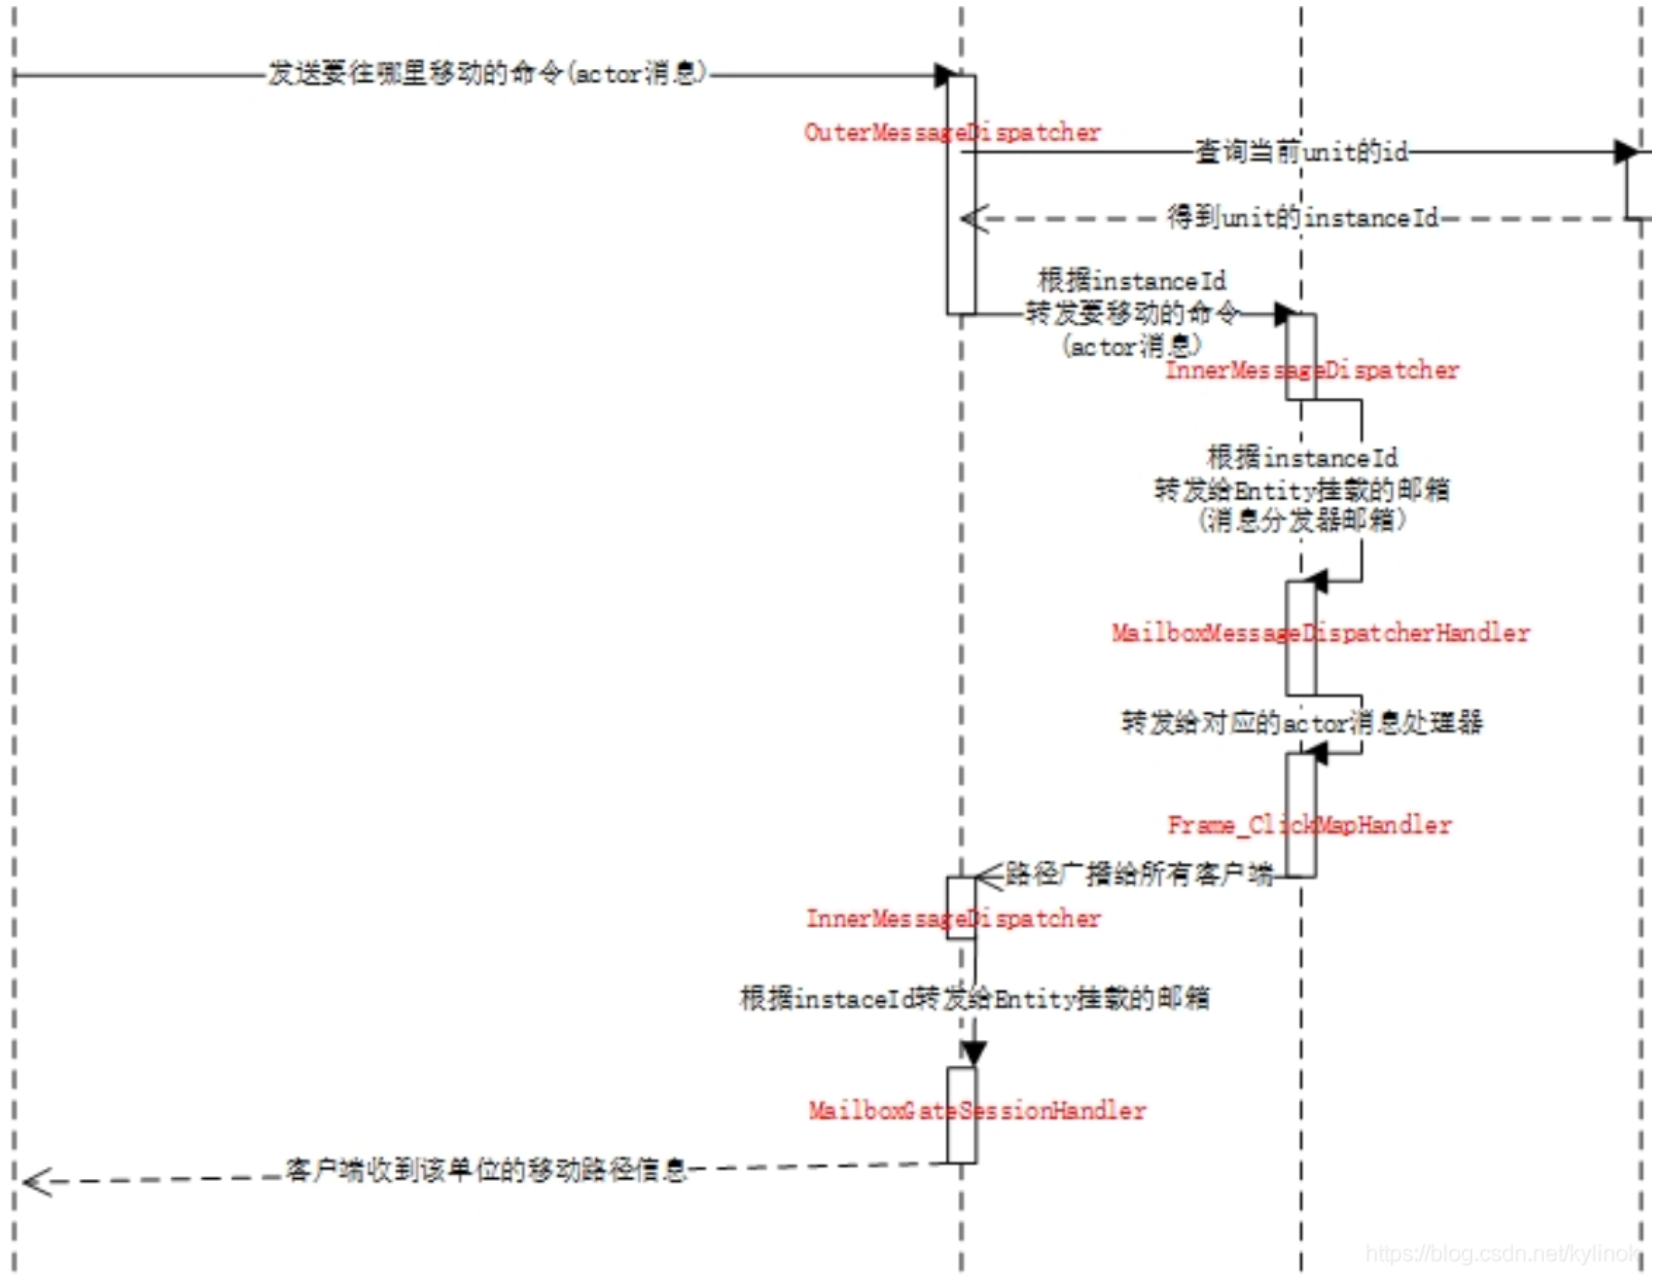
\includegraphics[width=.9\linewidth]{./pic/readme_20230219_102755.png}

\begin{itemize}
\item 爱亲爱的表哥,活宝妹一定要嫁的亲爱的表哥!!!,爱生活。活宝妹一定要嫁给亲爱的表哥。爱亲爱的表哥,活宝妹一定要嫁的亲爱的表哥!!!爱生活!!!
\end{itemize}
% Emacs 28.2 (Org mode 8.2.7c)
\end{document}